\chapter{Suchalgorithmen}
Ein Agent muss für ein bestimmtes Ziel die richtige Wahl von Aktion treffen und vorausplanen, eine Sequenz an Aktionen erstellen. Der Prozess für die Findung der Sequenz an Aktionen wird als Suche bezeichnet und durch Suchalgorithmen gefunden. Im Bereich der Suchalgorithmen wird zwischen informierten und uniformierten Algorithmen unterschieden. Informierte Algorithmen können dabei die Distanz zum Ziel schätzen, während uniformierte eine solche Schätzung nicht durchführen können. Sollte der Agent keine Informationen über seine Umwelt haben, so muss dierser mit Zufällen arbeiten. Mit Informationen über die Umwelt hat dieser aber die Möglichkeit den Weg zum Ziel über Suchalgorithmen zu finden.

\section{Suchproblem}
Ein Suchproblem wird definiert über einen Satz an möglichen Zuständen (\textit{states}), einen Ausgangszustand (\textit{initial state}), Zielzustände (\textit{goal states}), Aktionen (\textit{actions}), Übergangsmodel (\textit{transition model}) und Aktion-Kosten (\textit{action costs}).

Die Zustände beschreiben dabei die Umwelt und ein Ausgangszustand \textit{s} den Zustand des Agenten in dem der Agent startet. Ein Agent bekommt ein oder mehrere Ziele die in Zielzuständen beschrieben werden.
\begin{align*}
s = \{AtCover, BulletsAvailable, PlayerAlive\}
\end{align*}

Die Aktionen die ein Agent besitzt können in bestimmten Zuständen \textit{ACTIONS(s)} ausgeführt werden.
\begin{align*}
ACTIONS(BulletsAvailable) &= \{Shoot\} \\
ACTIONS(\lnot BulletsAvailable) &= \{Reload\}
\end{align*}

Ein Übergangsmodell \textit{TRANSITION(s,a) = s*} beschreibt dabei den resultierenden Zustand \textit{s*} der durch Aktionen \textit{a} im derzeitigen Zustand \textit{s} resultiert.
\begin{align*}
TRANSITIONS(BulletsAvailable, Shoot) &= \lnot PlayerAlive
\end{align*}

Durch eine Aktion-Kosten Funktion \textit{ACTION-COST(s,a,s*)} erhalten wir die Kosten einer Aktion\textit{a}, welche in einem Zustand \textit{s} ausgeführt werden und in einen neuen Zustand \textit{s*} resultieren.

%Die Lösung dabei ist die Sequenz an Aktionen die zum Zielzustand führen. Der Agent würde dieser Sequenz folgen und bei deterministischer Umwelt auch zum Zielzustand führen. Bei nichtdeterministischen Umwelten, wie Videospielen, werden so genannte closed-loop Systemen
Die Lösung für ein Suchproblem ist dabei ist die Sequenz an Aktionen, also der Plan der vom Ausgangszustand zum Zielzustand führen soll. Der gewählte Pfad sollte die geringsten Kosten von allen möglichen Lösungen haben und somit eine optimale Lösung darstellen. Der Satz an möglichen Zuständen kann dabei als Graph dargestellt werden. Dabei werden die Kanten als Aktionen und die Knoten als Zustände dargestellt.

\section{Suchalgorithmen}
Das Suchproblem soll mit seinen Informationen durch einen Suchalgorithmus gelöst werden. Ein Suchalgorithmus erzeugt für seine Suche einen Suchbaum aus dem Suchproblem. Wie beim Graphen sind in Suchbäumen Knoten Zustände und Kanten Aktionen, welche zu weiteren Zuständen führen. Der Wurzelknoten ist dabei der Ausgangszustand des Agenten. Der Suchbaum beschreibt dabei Pfade zu Knoten und zum Ziel und kann mehrere Pfade zu einem gegebenen Zustand haben, aber jeder Knoten im Baum hat einen eindeutigen Pfad zurück zur Wurzel.

\begin{figure}[h]
  \centering
  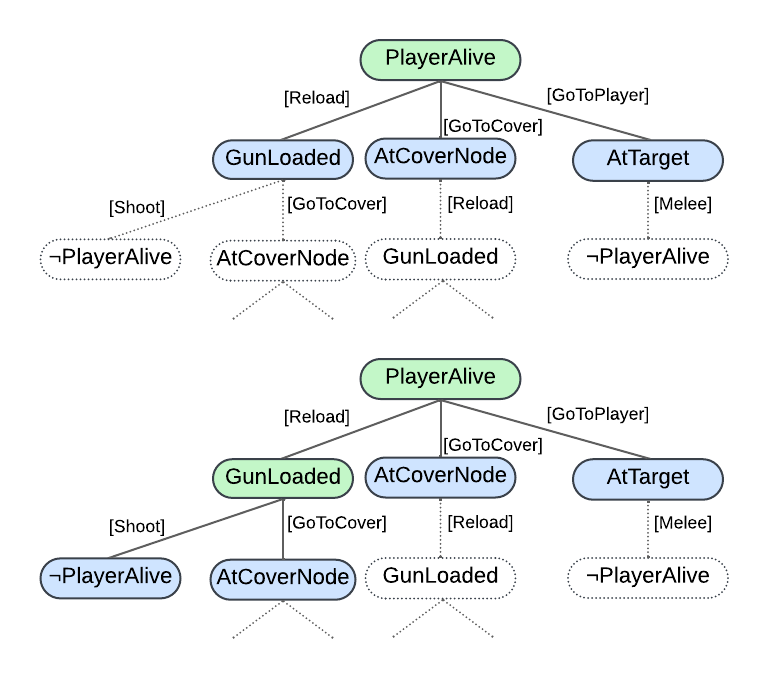
\includegraphics[width=15cm]{Suchalgorithmen/suchbaum2}
	\captionsetup{justification=justified, format=plain}
  \caption{Suchbaum: Fängt vom Ausgangszustand an und soll den Zielzustand $\lnot \textit{PlayerAlive}$ erreichen. Grüne Knoten sind expandierte Knoten, blaue Knoten sind offene gefundene Nachbarknoten und gestrichelte Knoten sind nicht entdeckte Knoten. Im Falle des Beispiels hat sich der Suchalgorithmus für den Knoten GunLoaded entschieden, da dieser optimaler als andere Nachbarknoten ist. Von dort aus ist der Zielzustand erreichbar und der Algorithmus würde eine Sequenz von Aktionen geben: \textit{[Reload,Shoot]}}
  %\label{Suchalgorithmen}
\end{figure}

\section{A* Algorithmus}

Gehört zu den heuristischen Suchverfahren. Wird oft für Routenplaner benutzt. So benutzt Godot 4.3 den A* Algorithmus für die Navigation. GOAP benutzt A* für das Suchen eines optimalen Pfades. A* ist ein vollständiger Algorithmus, er findet einen Pfad zur Lösung, wenn einer vorhanden ist. Die Kosten-Optimalität richtet sich nach einer Heuristik.Mit jeder Erweiterung des Pfades (n zu n*) steigen oder bleiben die g- Kosten gleich, was an den positiven Aktion-Kosten der Knoten liegt. g(n) + h(n) => g(n) + c(n,a,n‘) + h(n‘).

\subsection{A* Heuristik}
Eine Heuristik hat die Eigenschaften der Zulässigkeit und Konsistenz. Bei einer zulässigen Heuristik werden Kosten nue überschätzt. Also im Intervall [0,k] (k: tatsächliche Kosten).
Eine zunzulässige Heuristik kann zu nicht Kosten-Optimalen Pfaden führen. Eine konsistente Heuristik muss zulässig sein und die Dreiecksungleichung erfüllen. So ist die Abschätzung durch Luftlinie eine konsistente Heuristik. Die Dreiecksungleichung stellt die Regel, dass eine Seite nicht länger sein darf als die beiden anderen Seiten zusammen. Bezüglich Heuristik stellt sich daraus die Metrik: h(n) <= c(n,a,n‘) + h(n‘)
c(n,a,n‘): Aktion-kosten von n bis n‘
h(n‘): die Heuristik von n‘
Sollte eine Heuristik konsistent sein, so sind die besuchten Zustände optimal und müssen weder in eine offene noch in eine geschlossene Liste.
Mit einer inkonsistenten Heuristik können Pfade auftreten, welche denselben Zustand erreichen. Somit können mehrere Pfade mit unterschiedlichen Kosten aber selben Zustand in der offenen Liste auftreten, was zur höheren Zeit und Speicherkosten führt. Es gibt A* Implementationen, die dieses Problem berücksichtigen.

\begin{align}
Voraussetzung: f(Gs) &= g(h) + h(n); f(n) &= g(n) + h(n); h(n) \geq h*(n) \\
Behauptung: f(Gs) > f(n)
\end{align}
